%!TEX root = ../document.tex
\chapter{Architecture}\label{ch:architecture}

\begin{quotation}
“Some fantastic quote”
{\small\it --  }
\end{quotation}

This section describes the architecture designed for the browserCloud.js system. browserCloud.js was designed with with the Unix philosophy, that is, subtracting the unnecessary from a subsystem until it is constructed to perform one thing and one thing well, building more cohese abstractions through composition.

browserCloud.js was architectured to meet the following requirements:

\begin{itemize}
    \item \textbf{Membership management} - The system has to enable peers to join and leave a current network of browserCloud.js peers or a subset of it. A peer should only have the knowledge of a small of other peers in the network and be available to rail in any other peer that wants to be part of the P2P network.
    \item \textbf{Message routing} - Peers must have a way to communicate with every other peer in the network without the necessity of contacting a centralized service to do so. Messages should be routed between peers, having each peer knowing a subset of the network, guaranteeing in full coverage in this manner.
    \item \textbf{Job scheduling and results aggregation} - The discovery of computational resources must be performed using a distributed fashing, peers interact between each other to send tasks and retrieve the results for the peer executing the job.
    \item \textbf{Support dynamic runtime} - Provide flexibility for jobs being executed. This is delivered thanks to the dynamic runtime offered by by peers in browserCloud.js due to the fact that they are standard compliant web browsers and Javascript is the language used.
    \item \textbf{Reduced entrance cost to enable greater adoption} - Designed simple APIs, abstracting the complexity in favor of greater extendability.
\end{itemize}

The overview of the network architecture can be seen in Figure~\ref{fig:n-a-o}.

\begin{figure}[h!]
  \centering
  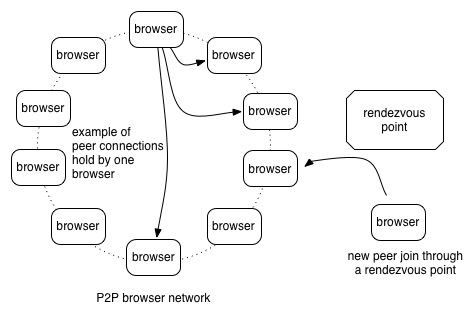
\includegraphics[width=0.7\textwidth]{figs/network-architecture-overview}
  \caption{browserCloud.js Network Architecture Overview}
  \label{fig:n-a-o}
\end{figure}

There are two different kind of actors in the system:

\begin{itemize}
    \item browser - The points on our network that will be able to issue jobs, execute tasks and route messages.
    \item rendezvous point - The only centralized component in this architecture, its purpose is for the clients to have a way to connect to the overlay network. 
\end{itemize}

\section{Interaction design details}

explain the algorithms in these sections

\subsection{Peer joins and leaves}

designed for this specific case
the state of the network is not stored but can be easily reconstructed

\subsection{Message routing}

Explain CHORD routing
Adaptable finger tables due to expensive Peer Connections

\subsection{Job Scheduling}

creation of gridlets, send and retrieve

\section{Architecture of the Software stack}

When it comes to software, we divided our browser application appliance into three separate and fundamental components, namely: Communication layer, Service router and Job scheduler, leaving also the opportunity for these to be extended. We can observe a overview of this architecture in Figure~\ref{fig:s-a-n-l}.

\begin{figure}[h!]
  \centering
  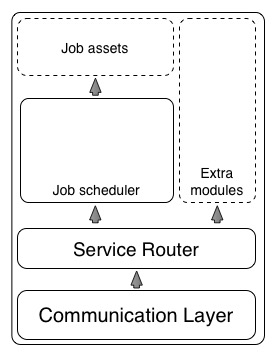
\includegraphics[width=0.4\textwidth]{figs/software-architecture-node-level}
  \caption{Software layers at the peer level}
  \label{fig:s-a-n-l}
\end{figure}


\subsection{Communication layer}

The communication layer is responsible for routing messages between peers and establish a connection with the rendezvous point to perform a peer join/leave. This means that the communication layer:

\begin{itemize}
    \item Holds the connections with other peers.
    \item Performs the necessarity logic for efficient routing.
    \item Keeps the peer connected to the network by updating its routing table as necessary
\end{itemize}

\subsection{Service router}

The Service router establishes a protocol for modules like the job scheduler to interact with the network of peers, it uses an event driven model, where modules can register listeners to events that happen on the network (such as a specific reception of a message) and react to it. It also offers the necessary API calls for the modules to send messages to the network.

Service router offers extensibility to browserCloud.js, similar to Job scheduler, other modules can be implemented to interact with the already established P2P network.

\subsection{Job scheduler}

The Job scheduler benefits the API of the Service router to implement its logic, this means that although a job scheduler was implemented to fit our design purposes, it could easily be replaced by another job scheduler with different offers and guarantees.

A job consists in the partition of tasks which are enriched with data and sent to other peers to be executed, this tasks, which can be represented as functions (job assets), can be defined in runtime, therefore giving a greater flexibility to the developer that is using this system to run the distributed job they want.

\section{API design details}

explain how the API works





\section{Summary}




CODE EXAMPLE:

\textit{sHolder pseudo-code}
\begingroup
\scriptsize
\begin{verbatim}
if(smallTask && available) {
  doIt(task, taskReport);
} else {
  requestNormalNodesToExecute(task, taskReport)
}
function taskReport(status){
  reportBack(status); // report to sKeeper
}
\end{verbatim}
\endgroup

FORMULA EXAMPLE

$ \textbf{reputation} = \alpha * log(uptime) + \beta * log(job completions) + $ \\
$          \gamma * log(network throughput) + \delta * log (CPU)$
\\
where: \\
\\
  $\alpha+ \beta+ \gamma+ \delta = 1$; \\
  $\alpha > \beta + \gamma + \delta$;  \\

\section*{Summary}
